\documentclass[main.tex]{subfiles}

\begin{document}

\chapter{Simplicial homotopy}
\label{ch:simplicial_homotopy}

\section{Homotopy of vertices}
\label{sec:homotopy_of_vertices}

\begin{definition}[homotopy of vertices]
  \label{def:homotopy_of_vertices}
  Let $S$ be a simplicial set. We say that $x$, $y \in K_{0}$ are \defn{homotopic} if there is an edge $f\colon x \to y$.
\end{definition}

\begin{theorem}
  \label{thm:homotopy_of_vertices_is_equivalence_relation}
  If $S = K$ is a Kan complex, the above notion is an equivalence relation.
\end{theorem}
\begin{proof}
  We have that $x$ is homotopic to $x$ because of the edge $s_{0}x$.

  Given $f\colon x \to y$ and $g\colon y \to z$, we can fill the following horn.
  \begin{equation*}
    \begin{tikzcd}[column sep=small]
      & y
      \arrow[dr, "g"]
      \\
      x
      \arrow[ur, "f"]
      \arrow[rr, dashed]
      && z
    \end{tikzcd}
  \end{equation*}
  This gives a homotopy from $x$ to $z$.

  Similarly, suppose we have a homotopy $x \to y$. Then filling the horn
  \begin{equation*}
    \begin{tikzcd}[column sep=small]
      & y
      \arrow[dr, dashed]
      \\
      x
      \arrow[ur, "f"]
      \arrow[rr, swap, "s_{0}x"]
      && x
    \end{tikzcd}
  \end{equation*}
  gives us a homotopy $y \to x$.
\end{proof}

Thus, we can think of partitioning a Kan complex into disconnected components.

\section{Homotopy of edges}
\label{sec:homotopy_of_edges}

We will often want to consider edges in a simplicial set up to some notion of homotopy.

\begin{definition}[homotopy of edges]
  \label{def:homotopy_of_edges}
  Let $f\colon x \to y$ and $g\colon x \to y$ be edges in some simplicial set $K$. We say that $f$ and $g$ are \defn{homotopic} if there exists a 2-simplex of the following form.
  \begin{equation*}
    \begin{tikzcd}[column sep=small]
      & w
      \arrow[dr, "s_{0}w"]
      \\
      v
      \arrow[ur, "f"]
      \arrow[rr, swap, "g"]
      && w
    \end{tikzcd}
  \end{equation*}
\end{definition}

Unfortunately, this is in general not an equivalence relation since it is not symmetric. It becomes one if we restrict our attention to Kan complexes. However, it turns out we will not have to make any use of outer horn fillers. This will be important later on.

\begin{theorem}
  \label{thm:homotopy_of_edges_is_equivalence_relation}
  For any set with inner horn fillers, that is fillers $\Lambda^{n}_{i} \to \Delta^{n}$ for $0 < i < n$, homotopy of edges is an equivalence relation. 
  
  In particular, it is an equivalence for any Kan complex $K$.
\end{theorem}
\begin{proof}
  First, we show reflexivity. For any edge $f$, the simplicial identities (\hyperref[thm:simplicial_identities]{Theorem~\ref*{thm:simplicial_identities}}) ensure that the degenerate simplex $\sigma_{f} = s_{1}f$ satisfies
  \begin{equation*}
    d_{1}\sigma_{f} = f,\qquad d_{2}\sigma_{f} = f,\qquad\text{and}\qquad d_{0}\sigma_{f} = s_{0}d_{0}f.
  \end{equation*}

  To see that it is symmetric, create from a 2-simplex
  \begin{equation*}
    \begin{tikzcd}[column sep=small]
      & y
      \arrow[dr, "s_{0}y"]
      \\
      x
      \arrow[ur, "f"]
      \arrow[rr, swap, "g"]
      && y
    \end{tikzcd}
  \end{equation*}
  the 1-skeleton of a 2-simplex whose front and back are as follows.
  \begin{equation*}
    \begin{tikzcd}
      y
      \arrow[r, "s_{0}y"]
      & y
      \arrow[d, "s_{0}y"]
      \\
      x
      \arrow[r, swap, "f"]
      \arrow[u, "f"]
      \arrow[ur, "g"]
      & y
    \end{tikzcd}
    \qquad
    \begin{tikzcd}
      y
      \arrow[r, "s_{0}y"]
      \arrow[dr, "s_{0}y"]
      & y
      \arrow[d, "s_{0}y"]
      \\
      x
      \arrow[r, swap, "f"]
      \arrow[u, "f"]
      & y
    \end{tikzcd}
  \end{equation*}

  This gives us the boundaries of four 1-simplices. Each of these can be filled except for the bottom simplex of the first diagram. Doing so gives us a 1-horn, which we can fill to find a 2-simplex as follows.
  \begin{equation*}
    \sigma' =
    \begin{tikzcd}[column sep=small]
      & y
      \arrow[dr, "s_{0}y"]
      \\
      x
      \arrow[ur, "g"]
      \arrow[rr, swap, "f"]
      && y
    \end{tikzcd}
  \end{equation*}

  This says precisely that $g \sim f$.

  To check transitivity, suppose we are given two simplices as follows.
  \begin{equation*}
    \begin{tikzcd}[column sep=small]
      & y
      \arrow[dr, "s_{0}y"]
      \\
      x
      \arrow[ur, "f"]
      \arrow[rr, swap, "g"]
      && y
    \end{tikzcd}
    \qquad\text{and}\qquad
    \begin{tikzcd}[column sep=small]
      & y
      \arrow[dr, "s_{0}y"]
      \\
      x
      \arrow[ur, "g"]
      \arrow[rr, swap, "h"]
      && y
    \end{tikzcd}
  \end{equation*}
  We can create a horn $\Lambda^{3}_{2} \to X$ as follows.
  \begin{equation*}
    \begin{tikzcd}
      y
      \arrow[r, "s_{0}y"]
      & y
      \arrow[d, "s_{0}y"]
      \\
      x
      \arrow[r, swap, "h"]
      \arrow[u, "f"]
      \arrow[ur, "g"]
      & y
    \end{tikzcd}
    \qquad
    \begin{tikzcd}
      y
      \arrow[r, "s_{0}y"]
      \arrow[dr, "s_{0}y"]
      & y
      \arrow[d, "s_{0}y"]
      \\
      x
      \arrow[r, swap, "h"]
      \arrow[u, "f"]
      & y
    \end{tikzcd}
  \end{equation*}

  Filling this gives what we want.
\end{proof}

\begin{theorem}
  \label{thm:equivalent_definition_of_homotopy_of_edges}
  Two edges $f$ and $g$ in a Kan complex $K$ are homotopic in the above sense if and only if there exists a square of the following form.
  \begin{equation*}
    \begin{tikzcd}
      v
      \arrow[r, "f"]
      \arrow[d, swap, "s_{0}v"]
      \arrow[dr]
      & w
      \arrow[d, "s_{0}w"]
      \\
      v
      \arrow[r, swap, "g"]
      & w
    \end{tikzcd}
  \end{equation*}
\end{theorem}
\begin{proof}
  Suppose we have a 2-simplex exhibiting $f$ and $g$ as homotopic. We can form a square by attaching the 2-simplex $s_{0}g$ as to the bottom.
  \begin{equation*}
    \begin{tikzcd}
      v
      \arrow[r, "f"]
      \arrow[d, swap, "s_{0}v"]
      \arrow[dr, "g"]
      & w
      \arrow[d, "s_{0}w"]
      \\
      v
      \arrow[r, swap, "g"]
      & w
    \end{tikzcd}
  \end{equation*}

  Given a square as above, call the bottom 2-simplex $\eta$ and the upper simplex $\mu$. Create the horn
  \begin{equation*}
    \begin{tikzcd}
      v
      \arrow[r, "s_{0}v"]
      \arrow[dr, "d_{1}\eta"]
      \arrow[d, swap, "g"]
      & v
      \arrow[d, "g"]
      \\
      w
      \arrow[r, swap, "s_{0}w"]
      & w
    \end{tikzcd}
    \qquad
    \begin{tikzcd}
      v
      \arrow[r, "s_{0}v"]
      \arrow[d, swap, "g"]
      & v
      \arrow[dl, swap, "g"]
      \arrow[d, "g"]
      \\
      w
      \arrow[r, swap, "s_{0}w"]
      & w
    \end{tikzcd}
  \end{equation*}
  where the top left simplex is $\eta$, the top right is $s_{0}g$, the bottom right is $s_{1}g$, and the bottom left is unfilled. Filling it, we find that $g \sim d_{1}\eta$. But $\mu$ exhibits $f \sim d_{1}\eta$, so $f \sim g$.
\end{proof}


\section{Homotopy of maps}
\label{sec:homotopy_of_maps}

\begin{definition}[homotopy]
  \label{def:homotopy}
  Let $f$, $g\colon B \to K$ be simplicial sets. A \defn{homotopy from $f$ to $g$} is a morphism
  \begin{equation*}
    H\colon \Delta^{1} \times B \to K
  \end{equation*}
  such that the restriction of $H$ to $\{0\} \times B$ is $f$, and the restriction of $H$ to $\{1\} \times B$ is $g$.

  In this case, we will write
  \begin{equation*}
    f \overset{H}{\simeq} g
  \end{equation*}

  To put it another way, $H$ is a homotopy above if the pullback along the inclusion $B \to \Delta^{1} \times B$ sending $\sigma \mapsto (0, \sigma)$ is equal to $f$, and similarly for $g$.
  \begin{equation*}
    \begin{tikzcd}[column sep=huge]
      \Delta^{0} \times B
      \arrow[d, swap, hookrightarrow, "\{0\} \times \id"]
      \arrow[rd, "f"]
      \\
      \Delta^{1} \times B
      \arrow[r, "H"]
      & K
      \\
      \Delta^{0} \times B
      \arrow[u, hookrightarrow, "\{1\} \times \id"]
      \arrow[ru, swap, "g"]
    \end{tikzcd}
  \end{equation*}
  Note that chasing elements around, this immediately implies that, for all $\sigma$,
  \begin{equation*}
    H(0, \sigma) = f(\sigma)\qquad\text{and}\qquad H(1, \sigma) = g(\sigma).
  \end{equation*}
\end{definition}

\begin{definition}[relative homotopy]
  \label{def:relative_homotopy}
  Suppose we are further given a monomorphism $i\colon A \to B$ making the following diagram commute.
  \begin{equation*}
    \begin{tikzcd}[column sep=huge]
      & B
      \arrow[dr, "f"]
      \\
      A
      \arrow[ur, "i"]
      \arrow[dr, swap, "i"]
      && K
      \\
      & B
      \arrow[ur, swap, "g"]
    \end{tikzcd}
  \end{equation*}
  Denote $f \circ i = g \circ i = u$. Then we say that $H$ is a \defn{homotopy relative to $A$} if the diagram
  \begin{equation*}
    \begin{tikzcd}
      \Delta^{1} \times B
      \arrow[r, "H"]
      & K
      \\
      \Delta^{1} \times A
      \arrow[r, swap, "\pi_{A}"]
      \arrow[u, "\id \times i"]
      & A
      \arrow[u, swap, "u"]
    \end{tikzcd}
  \end{equation*}
  commutes. We will write
  \begin{equation*}
    f \overset{H}{\simeq} g \rel{A}.
  \end{equation*}

  The intuitive meaning of this diagram is that $H$ leaves $A \subset B$ fixed. Indeed, again chasing elements around, we find that
  \begin{equation*}
    H(e, \sigma) = f(\sigma) = g(\sigma)
  \end{equation*}
  for all $\sigma \in A$ and $e = 0$, $1$.

\end{definition}

We would like to use homotopy to define an equivalence relation on maps of simplicial sets. However, in a general simplicial set this is impossible. Consider the maps
\begin{equation*}
  \iota_{0},\ \iota_{1}\colon \Delta^{0} \to \Delta^{1}.
\end{equation*}
which send the point to the zeroth and first vertices. The morphisms $\iota_{0}$ and $\iota_{1}$ satisfy
\begin{equation*}
  \iota_{0} \simeq  \iota_{1},
\end{equation*}
since $H = \id_{\Delta^{1}}$ makes the following diagram commute.
\begin{equation*}
  \begin{tikzcd}[column sep=huge]
    \Delta^{0} \times \Delta^{0} = \Delta^{0}
    \arrow[d, swap, "d^{1} \times \id"]
    \arrow[rd, "\iota_{0}"]
    \\
    \Delta^{1} \times \Delta^{0} = \Delta^{1}
    \arrow[r, "H = \id_{\Delta^{1}}"]
    & \Delta^{1}
    \\
    \Delta^{0} \times \Delta^{0} = \Delta^{0}
    \arrow[ru, swap, "\iota_{1}"]
    \arrow[u, "d^{0} \times \id"]
  \end{tikzcd}
\end{equation*}
However, there is no morphism $H\colon \Delta^{1} \to \Delta^{1}$ which sends $0 \mapsto 1$ and $1 \mapsto 0$, so there does not exist any $H$ such that
\begin{equation*}
  \iota_{1} \overset{H}{\simeq} \iota_{0}.
\end{equation*}

The way out of this is to specialize to Kan complexes.

\begin{proposition}
  \label{prop:relative_homotopy_defines_equiv_relation_on_kan_complex}
  Let $i\colon A \to B$ be a monomorphism of simplicial sets, let $K$ be a Kan complex, and let $u\colon A \to K$ be a morphism. Then the relation \emph{is homotopic relative to $A$} defines an equivalence relation on the set
  \begin{equation*}
    \{ f\colon B \to K \mid f \circ i = u \}.
  \end{equation*}
\end{proposition}
\begin{proof}
  By \hyperref[note:morphisms_are_vertices_of_mapping_space]{Note~\ref*{note:morphisms_are_vertices_of_mapping_space}}, we can think of $u$ as a map $\Delta^{0} \to \Maps(A, K)$ which picks out $u$ as a zero-simplex.

  Consider the pullback square
  \begin{equation*}
    \begin{tikzcd}
      \Maps(B, K)^{u}
      \arrow[r]
      \arrow[d]
      & \Maps(B, K)
      \arrow[d, "{\Maps(i, \id_{K})}"]
      \\
      \Delta^{0}
      \arrow[r, swap, "u"]
      & \Maps(A, K)
    \end{tikzcd}
  \end{equation*}

  By \hyperref[cor:maps_functor_preserves_kan_fibrations_in_first_slot]{Corollary~\ref*{cor:maps_functor_preserves_kan_fibrations_in_first_slot}}, the map $\Maps(i, \id_{K})$ is a Kan fibration. Thus, since Kan fibrations are saturated (hence closed under pullback), we have that the induced map $\Maps(B, K)^{u} \to \{u\}$ is also a Kan fibration. But by \hyperref[cor:kan_fibration_to_point_is_kan_complex]{Corollary~\ref*{cor:kan_fibration_to_point_is_kan_complex}}, this means that $\Maps(B, K)^{u}$ is a Kan complex.

  The elements of $\Maps(B, K)^{u}_{0}$ are ordered pairs $(u, f) \in \{u\} \times \SSet(B, K)$ such that $u = i \circ f$. That is, $\Maps(B, K)^{u}_{0}$ consists of those morphisms $B \to K$ which agree with $u$ when restricted to $A$ along $i$.

  Thus, showing that homotopy between maps $B \to K$ relative to $A$ is an equivalence relation is the same as showing homotopy between vertices of the Kan complex $\Maps(B, K)^{u}$ is an equivalence relation, which is true by \hyperref[thm:homotopy_of_edges_is_equivalence_relation]{Theorem~\ref*{thm:homotopy_of_edges_is_equivalence_relation}}.
\end{proof}

\section{Homotopy groups}
\label{sec:homotopy_groups}

\begin{definition}[homotopy group]
  \label{def:homotopy_group}
  Let $K$ be a Kan complex. Define the \defn{zeroth homotopy group of $K$}, denoted $\pi_{0}(K)$, to be the set of homotopy classes of vertices of $K$. This is well-defined by \hyperref[thm:homotopy_of_vertices_is_equivalence_relation]{Theorem~\ref*{thm:homotopy_of_vertices_is_equivalence_relation}}.

  For $n \geq 1$, define the \defn{$n$th homotopy group of $K$ at $v$}, denoted $\pi_{n}(K, v)$, to be the set of homotopy classes of $n$-simplices $\alpha\colon \Delta^{n} \to K$ relative to the inclusion $\partial\Delta^{n} \hookrightarrow \Delta^{n}$, such that the following diagram commutes.
  \begin{equation*}
    \begin{tikzcd}
      \Delta^{n}
      \arrow[r, "\alpha"]
      & X
      \\
      \partial\Delta^{n}
      \arrow[r]
      \arrow[u, hookrightarrow]
      & \Delta^{0}
      \arrow[u, swap, hookrightarrow, "v"]
    \end{tikzcd}
  \end{equation*}
  This diagram says precisely that the boundary of $\Delta^{n}$ is collapsed to the point $v$.
\end{definition}

\begin{definition}
  \label{def:composition_in_homotopy_groups}
  Let $\alpha$, $\beta\colon \Delta^{n} \to K$ be $n$-simplices whose boundaries are trivial. Denote their equivalence classes by $[\alpha]$ and $[\beta]$ respective. Define their \defn{composition}, denoted $[\alpha]\cdot[\beta]$ as follows. First, define an inner $(n+1)$-horn with faces
  \begin{equation*}
    (\overbrace{\{v\}, \cdots, \{v\}}^{n-1}, \alpha, -, \beta).
  \end{equation*}
  This has a filler $\sigma$ such that
  \begin{equation*}
    \partial\sigma = (\{v\}, \cdots, \{v\}, \alpha, d_{n}\sigma, \beta)
  \end{equation*}
  Define $[\alpha]\cdot[\beta] = [d_{n}\sigma]$.

  It remains to check that this composition is well-defined.
\end{definition}

\begin{proposition}
  \label{prop:multiplication_in_homotopy_groups_well_defined}
  The composition defined above is well-defined, i.e.\ if $\alpha' \overset{H}{\simeq} \alpha$ and $\beta' \overset{H'}{\simeq} \beta$, then $[\alpha']\cdot[\beta'] = [\alpha]\cdot[\beta]$.
\end{proposition}
\begin{proof}[Sketch of proof]
  We have homotopies between the $n$-simplices we want to multiply,
  \begin{equation*}
    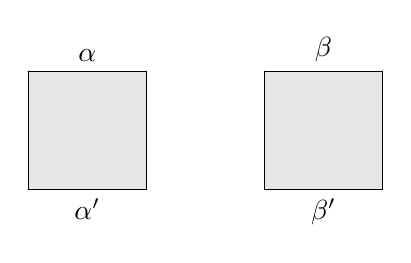
\begin{tikzpicture}[dot/.style={draw,circle,minimum size=1mm,inner sep=0pt,outer sep=0pt,fill=black}, line join = round, scale=1.5, line cap = round]
      \coordinate (a1) at (0,1);
      \coordinate (a2) at (1,1);
      \coordinate (a3) at (0,0);
      \coordinate (a4) at (1,0);

      \coordinate (b1) at (2,1);
      \coordinate (b2) at (3,1);
      \coordinate (b3) at (2,0);
      \coordinate (b4) at (3,0);

      \draw [fill=gray, fill opacity=0.2] (a1) -- (a2) -- (a4) -- (a3) -- cycle;
      \draw (a1) -- node[midway, above]{$\alpha$} ++(1,0) -- (a2);
      \draw (a1) -- (a3);
      \draw (a2) -- (a4);
      \draw (a3) -- node[midway, below]{$\alpha'$} ++(1,0) -- (a4);

      \draw [fill=gray, fill opacity=0.2] (b1) -- (b2) -- (b4) -- (b3) -- cycle;
      \draw (b1) -- node[midway, above]{$\beta$} ++(1,0) -- (b2);
      \draw (b1) -- (b3);
      \draw (b2) -- (b4);
      \draw (b3) -- node[midway, below]{$\beta'$} ++(1,0) -- (b4);
    \end{tikzpicture}
  \end{equation*}
  which we extend to a homotopy between the horns defining our multiplication law.
  \begin{equation*}
    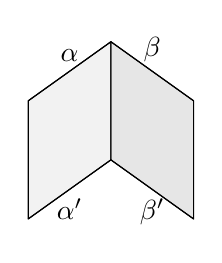
\begin{tikzpicture}[dot/.style={draw,circle,minimum size=1mm,inner sep=0pt,outer sep=0pt,fill=black}, line join = round, scale=1.5, line cap = round]
      \coordinate (a1) at (0,1);
      \coordinate (c1) at (0.7,1.5);
      \coordinate (b1) at (1.4,1);

      \coordinate (a2) at (0,0);
      \coordinate (c2) at (0.7,0.5);
      \coordinate (b2) at (1.4,0);

      \draw [fill=lightgray, fill opacity=0.2] (a1) -- (c1) -- (c2) -- (a2) -- cycle;
      \draw [fill=gray, fill opacity=0.2] (c1) -- (b1) -- (b2) -- (c2) -- cycle;
      \draw (a1) -- node[midway, above]{$\alpha$} ++(0.7,0.5) -- (c1);
      \draw (a2) -- node[midway, below]{$\alpha'$} ++(0.7,0.5) -- (c2);
      \draw (c1) -- node[midway, above]{$\beta$} ++(0.7,-0.5) -- (b1);
      \draw (c2) -- node[midway, below]{$\beta'$} ++(0.7,-0.5) -- (b2);
    \end{tikzpicture}
  \end{equation*}
  These horns have fillers, giving us the result of our multiplication.
  \begin{equation*}
    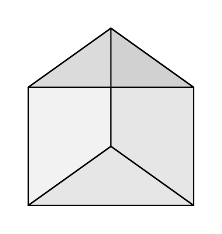
\begin{tikzpicture}[dot/.style={draw,circle,minimum size=1mm,inner sep=0pt,outer sep=0pt,fill=black}, line join = round, scale=1.5, line cap = round]
      \coordinate (a1) at (0,1);
      \coordinate (c1) at (0.7,1.5);
      \coordinate (b1) at (1.4,1);

      \coordinate (a2) at (0,0);
      \coordinate (c2) at (0.7,0.5);
      \coordinate (b2) at (1.4,0);

      \draw [fill=lightgray, fill opacity=0.2] (a1) -- (c1) -- (c2) -- (a2) -- cycle;
      \draw [fill=gray, fill opacity=0.2] (c1) -- (b1) -- (b2) -- (c2) -- cycle;
      \draw [fill=gray, fill opacity=0.2] (a1) -- (c1) -- (b1) -- cycle;
      \draw [fill=gray, fill opacity=0.2] (a2) -- (c2) -- (b2) -- cycle;
    \end{tikzpicture}
  \end{equation*}
  Using the general theory of anodyne morphisms, we can extend our homotopy between the horns to a homotopy between the full filled simplices.
  \begin{equation*}
    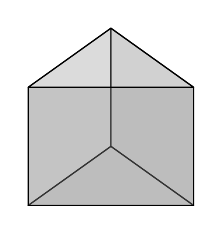
\begin{tikzpicture}[dot/.style={draw,circle,minimum size=1mm,inner sep=0pt,outer sep=0pt,fill=black}, line join = round, scale=1.5, line cap = round]
      \coordinate (a1) at (0,1);
      \coordinate (c1) at (0.7,1.5);
      \coordinate (b1) at (1.4,1);

      \coordinate (a2) at (0,0);
      \coordinate (c2) at (0.7,0.5);
      \coordinate (b2) at (1.4,0);

      \draw [fill=lightgray, fill opacity=0.2] (a1) -- (c1) -- (c2) -- (a2) -- cycle;
      \draw [fill=gray, fill opacity=0.2] (c1) -- (b1) -- (b2) -- (c2) -- cycle;
      \draw [fill=gray, fill opacity=0.2] (a1) -- (c1) -- (b1) -- cycle;
      \draw [fill=gray, fill opacity=0.2] (a2) -- (c2) -- (b2) -- cycle;
      \draw [fill=gray, fill opacity=0.4] (a1) -- (b1) -- (b2) -- (a2) -- cycle;
    \end{tikzpicture}
  \end{equation*}
  Restricting to the filled faces gives us a homotopy between the result of multiplication.
  \begin{equation*}
    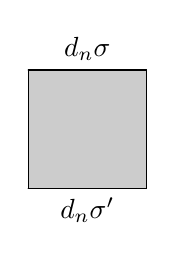
\begin{tikzpicture}[dot/.style={draw,circle,minimum size=1mm,inner sep=0pt,outer sep=0pt,fill=black}, line join = round, scale=1.5, line cap = round]
      \coordinate (a1) at (0,1);
      \coordinate (a2) at (1,1);
      \coordinate (a3) at (0,0);
      \coordinate (a4) at (1,0);

      \draw [fill=gray, fill opacity=0.4] (a1) -- (a2) -- (a4) -- (a3) -- cycle;
      \draw (a1) -- node[midway, above]{$d_{n}\sigma$} ++(1,0) -- (a2);
      \draw (a1) -- (a3);
      \draw (a2) -- (a4);
      \draw (a3) -- node[midway, below]{$d_{n}\sigma'$} ++(1,0) -- (a4);
    \end{tikzpicture}
  \end{equation*}
\end{proof}
\begin{proof}
  By definition, we have an $(n+1)$-simplices $\sigma$ and $\sigma'$ such that
  \begin{equation*}
    \partial\sigma = (\{v\}, \ldots, \{v\}, \alpha, d_{n}\sigma, \beta)
  \end{equation*}
  and
  \begin{equation*}
    \partial\sigma' = (\{v\}, \ldots, \{v\}, \alpha', d_{n}\sigma', \beta').
  \end{equation*}

  We need to show that $d_{n}\sigma \simeq d_{n} \sigma'$.

  First, we construct a homotopy between the horns
  \begin{equation*}
    \eta = (\{v\}, \ldots, \{v\}, \alpha, -, \beta) \qquad\text{and}\qquad \eta' = (\{v\}, \ldots, \{v\}, \alpha', -, \beta').
  \end{equation*}
  By the distributive law for products and coproducts
  \begin{equation*}
    A \times (B \amalg C) \simeq (A \times B) \amalg (A \times C),
  \end{equation*}
  a homotopy between horns $\Lambda^{n+1}_{i} \to K$ consists of a homotopy for each face. Therefore, we can choose our homotopy $H''$ to have components $(\id_{v}, \ldots, \id_{v}, H, -, H')$. This gives us a map $\Delta^{1} \times \Lambda^{n+1}_{n} \to K$. Our fillers give us two maps $\sigma$, $\sigma'\colon \Delta^{n+1} \to K$, which we can view as a map $\partial\Delta^{1} \times \Delta^{n+1} \to K$. This gives us the following commutative diagram
  \begin{equation*}
    \begin{tikzcd}
      \partial \Delta^{1} \times \Lambda^{n+1}_{n}
      \arrow[r, hookrightarrow]
      \arrow[d, hookrightarrow]
      & \partial \Delta^{1} \times \Delta^{n+1}
      \arrow[d, "({\sigma, \sigma'})"]
      \\
      \Delta^{1} \times \Lambda^{n+1}_{n}
      \arrow[r, "H''"]
      & K
    \end{tikzcd}
  \end{equation*}
  This gives us a map
  \begin{equation*}
    h\colon \Delta^{1} \times \Lambda^{n+1}_{n} \coprod_{\partial \Delta^{1} \times \Lambda^{n+1}_{n}} \partial \Delta^{1} \times \Delta^{n+1} \to K.
  \end{equation*}

  Note that by \hyperref[eg:boundary_filling_times_horn_filling_is_anodyne]{Example~\ref*{eg:boundary_filling_times_horn_filling_is_anodyne}}, we get an anodyne extension
  \begin{equation*}
    \Delta^{1} \times \Lambda^{n+1}_{n} \coprod_{\partial \Delta^{1} \times \Lambda^{n+1}_{n}} \partial \Delta^{1} \times \Delta^{n+1} \hookrightarrow \Delta^{1} \times \Delta^{n}.
  \end{equation*}
  This means that (by \hyperref[cor:kan_fibration_to_point_is_kan_complex]{Corollary~\ref*{cor:kan_fibration_to_point_is_kan_complex}}) we can find a lift for the following diagram.
  \begin{equation*}
    \begin{tikzcd}
      \Delta^{1} \times \Lambda^{n+1}_{n} \coprod_{\partial \Delta^{1} \times \Lambda^{n+1}_{n}} \partial \Delta^{1} \times \Delta^{n+1}.
      \arrow[r, "h"]
      \arrow[d, hookrightarrow]
      & K
      \\
      \Delta^{1} \times \Delta^{n+1}
      \arrow[ur, dashed, swap, "\exists I"]
    \end{tikzcd}
  \end{equation*}

  Restricting $I$ to the $n$th face of $\Delta^{n+1}$ gives us a homotopy
  \begin{equation*}
    \Delta^{1} \times \Delta^{n} \to K
  \end{equation*}
  as required.
\end{proof}

\begin{theorem}
  \label{thm:homotopy_groups_are_actual_groups}
  Let $K$ be a Kan complex, and let $v \in K_{0}$ be a vertex of $K$. Then the multiplication from \hyperref[def:composition_in_homotopy_groups]{Definition~\ref*{def:composition_in_homotopy_groups}} makes $\pi_{n}(K, v)$ into a group for $n \geq 1$.
\end{theorem}
\begin{proof}
  First we check associativity. Let $\alpha$, $\beta$, $\gamma \colon \Delta^{n} \to K$ be $n$-simplices with trivial boundary, representing elements $[\alpha]$, $[\beta]$, $[\gamma] \in \pi_{n}(K, v)$. By definition, we get an $(n+1)$-simplex $\sigma_{n-1}$ such that
  \begin{equation*}
    \partial \sigma_{n-1} = (v, v, \ldots, v, \alpha, d_{n} \sigma_{n-1}, \beta).
  \end{equation*}
  giving us the result of the multiplication $[\alpha]\cdot[\beta] = [d_{n}\sigma_{n-1}]$.

  Similarly, we have some $\sigma_{n+2}$ such that
  \begin{equation*}
    \partial\sigma_{n+2} = (v, v, \ldots, v, \beta, d_{n} \sigma_{n+2}, \gamma)
  \end{equation*}
  so $[\beta]\cdot[\gamma] = [d_{n} \sigma_{n+2}]$.

  Form from these a simplex $\sigma_{n+1}$ with boundary
  \begin{equation*}
    \partial \sigma_{n+1} = (v, v, \ldots, v, d_{n} \sigma_{n-1}, d_{n}\sigma_{n+1}, \gamma)
  \end{equation*}
  giving us the result of the multiplication $([\alpha]\cdot[\beta])\cdot[\gamma] = [d_{n}\sigma_{n-1}]\cdot[\gamma] = [d_{n} \sigma_{n+1}]$.

  These simplices fit together to give a horn
  \begin{equation*}
    \Lambda^{n+2}_{n} \to K
  \end{equation*}
  with boundary
  \begin{equation*}
    (v, v, \ldots, v, \sigma_{n-1}, -, \sigma_{n+1}, \sigma_{n+2}).
  \end{equation*}
  Filling this gives an $(n+1)$-simplex $\sigma$ with boundary
  \begin{equation*}
    \partial\sigma = (v, v, \ldots, v, \sigma_{n-1}, d_{n}\sigma, \sigma_{n+1}, \sigma_{n+2}).
  \end{equation*}

  Using the simplicial identities, we find
  \begin{align*}
    \partial d_{n} \sigma &= (d_{0}d_{n}\sigma, d_{1}d_{n}\sigma, \ldots, d_{n-2}d_{n}\sigma, d_{n-1}d_{n}\sigma, d_{n}d_{n}\sigma, d_{n+1}d_{n}\sigma) \\
    &= (d_{n-1}d_{0}\sigma, d_{n-1}d_{1}\sigma, \ldots, d_{n-1}d_{n-2}\sigma, d_{n-1}d_{n-1}\sigma, d_{n}d_{n+1}\sigma, d_{n}d_{n+2}\sigma) \\
    &= (v, v, \ldots, v, \alpha, d_{n}\sigma_{n+1}, d_{n}\sigma_{n+2}).
  \end{align*}
  This is an $n$-simplex exhibiting $[\alpha]\cdot[d_{n}\sigma_{n-2}] = [d_{n}\sigma_{n+1}]$.

  Thus, we have
  \begin{align*}
    ([\alpha]\cdot[\beta])\cdot[\gamma] &= [d_{n}\sigma_{n-1}]\cdot[\gamma] \\
    &= [d_{n} \sigma_{n+1}] \\
    &= [\alpha] \cdot [d_{n}\sigma_{n+2}] \\
    &= [\alpha] \cdot ([\beta]\cdot[\gamma]).
  \end{align*}

  The degenerate $n$-simplex $v$ functions as a unit on the left because there exists an $(n+1)$-horn $s_{n}\omega$ with
  \begin{align*}
    \partial(s_{n}\omega) &= (d_{0}s_{n}\omega, \ldots, d_{n-1}s_{n}\omega, d_{n}s_{n}\omega, d_{n+1}s_{n}\omega) \\
    &=(s_{n-1}d_{0}\omega, \ldots, s_{n-1}d_{n-1}\omega, \omega, \omega) \\
    &= (v, \ldots, v, v, \omega, \omega),
  \end{align*}
  so $[e]\cdot[\omega] = [\omega]$. 

  It functions as a unit on the right because of $s_{n-2}\omega$.

  Furthermore.
\end{proof}

We would like $\pi_{0}(K)$ and $\pi_{n}(K, v)$ to be the simplicial analogs of the topological notions of homotopy groups. Recall that we can turn any simplicial set into a topological space via the geometric realization functor $\abs{\cdot}$. Therefore, one would hope that the simplicial homotopy groups would agree with the homotopy groups of the geometrical realization. At least for $\pi_{o}$ this turns out to be the case.

\begin{theorem}
  For any Kan complex $K$, we have $\pi_{0}(K) \simeq \pi_{0}(K)$ as sets.
\end{theorem}
\begin{proof}
  Define a map $K_{0} \to \abs{K}$ sending $v \to \abs{v}$.

  Suppose $v \sim v'$ in $K$. Then there is an edge $f$ between $v$ and $k$. Applying $\abs{\cdot}$, we find an edge $\abs{v} \to \abs{v'}$. Thus, the map above respects equivalence classes, and descends to a map $\pi_{0}(K) \to \pi_{0}(\abs{K})$.

  Now some homotopy stuff I don't understand.
\end{proof}

\begin{theorem}
  Let $p\colon K \to S$ be a Kan fibration. Let $v$ be a vertex of $K$, and let $w = p(v)$. Let $F$ be the fiber over $w$ given by the following pullback equare.
  \begin{equation*}
    \begin{tikzcd}
      F
      \arrow[r]
      \arrow[d]
      & K
      \arrow[d, "p"]
      \\
      \{w\}
      \arrow[r, hookrightarrow]
      & S
    \end{tikzcd}
  \end{equation*}

  There is the following long exact sequence.
  \begin{equation*}
    \cdots \longrightarrow \pi_{n+1}(K, v) \longrightarrow \pi_{n}(F, v) \longrightarrow \pi_{n}(K, v) \longrightarrow \pi_{n}(S, w) \longrightarrow \pi_{n-1}(F, v) \longrightarrow \cdots
  \end{equation*}
\end{theorem}

\end{document}
